%%________________________________________________________________________
%% LEIM | PROJETO
%% 2026
%% Relatório - Capítulos 4, 5 e 6
%%________________________________________________________________________

%%________________________________________________________________________
\chapter{Implementação do Modelo}
\label{ch:implementacaoDoModelo}
%%________________________________________________________________________

Neste capítulo, descrevemos a arquitetura e detalhes técnicos de concretização da aplicação nativa desenvolvida para Android utilizando a linguagem Kotlin e o ecossistema Jetpack Compose.

\begin{figure}[h]
   \centering
   \includegraphics[width=\linewidth]{figuras/arquitetura minimalista.png}
   \caption{Diagrama da arquitetura do projeto}
   \label{fig:umlClasses}
\end{figure}


%%________________________________________________________________________
\section{Arquitetura e Fluxo de Visão por Computador}
\label{sec:arquiteturaMobile}
%%________________________________________________________________________

Antes de se chegar a esta arquitetura, foi construído um protótipo em Python (OpenCV e MediaPipe), a correr num computador, para validar a viabilidade da deteção de pose e da lógica de contagem de repetições. Confirmada a abordagem, mas reconhecendo que manter o motor de deteção como um sistema à parte do produto final traria complexidade de integração sem benefício real, decidiu-se reescrever a lógica de produção nativamente em Kotlin, diretamente integrada na app Android; o protótipo permanece no repositório (\texttt{03\_Implementacao/POC\_Python}) como prova de conceito histórica.

A aplicação segue a arquitetura \textbf{MVVM (Model-View-ViewModel)}, escolhida por separar claramente a lógica de negócio (avaliação de forma, máquina de estados) da camada de interface, facilitando a testabilidade e alinhando-se com a gestão de estado reativa e declarativa do Jetpack Compose. O Compose foi adotado para toda a interface por reduzir o código repetitivo face ao sistema tradicional de \textit{Views} em XML e por permitir desenhar os gráficos de progresso do painel analítico (Secção \ref{sec:testesAnalitica}) diretamente em Canvas, sem depender de bibliotecas de gráficos de terceiros. A captura de imagem recorre à biblioteca CameraX em vez da Camera2 API de baixo nível, por abstrair variações de hardware entre fabricantes e reduzir a complexidade de gestão do ciclo de vida da câmara. O pipeline de processamento de imagem da câmara assenta na seguinte estrutura:
\begin{enumerate}
    \item \textbf{Captura de Imagem (CameraX):} Configura a câmara frontal do dispositivo móvel para obter frames no formato RGBA\_8888 de forma contínua e assíncrona;
    \item \textbf{Pré-processamento:} Roda o bitmap da frame de acordo com a rotação física do dispositivo e aplica um efeito de espelho (\textit{mirror}) para que a experiência do utilizador seja intuitiva;
    \item \textbf{Scheduler do MediaPipe:} O motor BlazePose opera em modo \textit{Live Stream}, com a estratégia de descarte de frames do CameraX (detalhada adiante) a garantir que a cadência de inferência não fica presa a frames antigas;
    \item \textbf{Lógica de Negócio Local:} Após a inferência, a lista de 33 coordenadas normalized 3D é canalizada para a classe Kotlin correspondente ao exercício ativo.
\end{enumerate}

O MediaPipe Pose Landmarker segue a arquitetura leve de duas fases descrita por Bazarevsky et al. \cite{Bazarevsky_BlazePose_2020}: um detetor de corpo inteiro localiza a região de interesse do utilizador apenas na primeira frame (ou sempre que o rastreio é perdido), e um modelo de rastreio estima os 33 landmarks a partir dessa região em cada frame seguinte, evitando repetir a deteção completa do corpo em todas as frames e reduzindo o custo computacional.

Este projeto utiliza especificamente a variante \texttt{pose\_landmarker\_lite}, a mais leve das três disponibilizadas pela Google (Lite, Full, Heavy), que os próprios autores do BlazePose reportam atingir até 31 frames por segundo num Google Pixel 2 \cite{Bazarevsky_BlazePose_2020}, favorecendo a fluidez em tempo real face à precisão adicional das variantes mais pesadas. Não é imposta nenhuma resolução ou frame rate fixos: o \texttt{ImageAnalysis} do CameraX é configurado com a estratégia \texttt{STRATEGY\_KEEP\_ONLY\_LATEST}, que descarta frames antigas em fila e analisa sempre a mais recente, deixando a cadência efetiva de inferência adaptar-se automaticamente à capacidade de cada dispositivo, com as frames entregues ao MediaPipe no formato \texttt{RGBA\_8888} através da câmara frontal (\texttt{CameraSelector.DEFAULT\_FRONT\_CAMERA}).


%%________________________________________________________________________
\section{Módulos de Código Principais}
\label{sec:modulosCodigo}
%%________________________________________________________________________

O processamento cinemático e as interações de treino apoiam-se num conjunto de classes Kotlin que concretizam diretamente o modelo apresentado no Capítulo \ref{ch:modeloProposto}:
\begin{itemize}
    \item \textbf{\texttt{AngleCalculator}:} Implementa a fórmula geométrica $\theta = \arccos\left(\vec{BA} \cdot \vec{BC} / (|\vec{BA}||\vec{BC}|)\right)$ apresentada na Secção \ref{sec:abordagem}, calculada a partir das coordenadas $x,y$ de três landmarks;
    \item \textbf{\texttt{ExerciseConfig}:} Estrutura de dados que armazena, por exercício, os limiares definidos na Secção \ref{sec:fundamentos} (limiar ideal, limiar de contagem, limiar de extensão) e os intervalos de cadência ideal usados na Secção \ref{sec:abordagem};
    \item \textbf{\texttt{RepPhaseTracker}:} Implementa a máquina de estados \texttt{AT\_TOP}/\texttt{DESCENDING}/\texttt{ASCENDING} da Figura \ref{fig:stateMachine}, medindo a duração em milissegundos das fases descendente (excêntrica) e ascendente (concêntrica) e registando a amplitude de movimento mínima da articulação central durante a repetição;
    \item \textbf{\texttt{FormEvaluator}:} Implementa as penalizações de score descritas na Secção \ref{sec:abordagem} e devolve strings estruturadas de correção física;
    \item \textbf{\texttt{TTSHelper}:} Wrapper do motor de síntese de voz nativo do Android. Implementa um limite temporal de repetição (cooldown) para evitar saturação acústica do atleta, com exceção da conclusão de repetições e números de contagens, que são pronunciados de imediato;
    \item \textbf{\texttt{OverlayView}:} Vista customizada que desenha o esqueleto corporal do utilizador e elementos informativos (HUD) em neon, incluindo avisos de calibração ("Note: Audio guidance will be used...").
\end{itemize}

Cada um dos quatro exercícios (Agachamento, Flexão de Braços, Lunge e Prancha) é implementado numa classe própria (\texttt{SquatExercise}, \texttt{PushUpExercise}, \texttt{LungeExercise} e \texttt{PlankExercise}, respetivamente), todas a implementar uma interface comum \texttt{Exercise}. Os três primeiros combinam \texttt{RepPhaseTracker} e \texttt{FormEvaluator} exatamente como descrito acima; a Prancha, por avaliar uma postura estática e não uma repetição (Secção \ref{sec:abordagem}), não usa nenhuma das duas classes, implementando antes a sua própria lógica de acumulação de tempo sob tensão e desvio médio do ângulo. Cada repetição concluída pelos três primeiros exercícios (ou cada segmento de prancha concluído) gera uma instância de \texttt{RepMetrics}, guardada no histórico do exercício (\texttt{repHistory}). A Figura \ref{fig:umlClasses} resume as relações entre estas classes.

\begin{figure}[h]
   \centering
   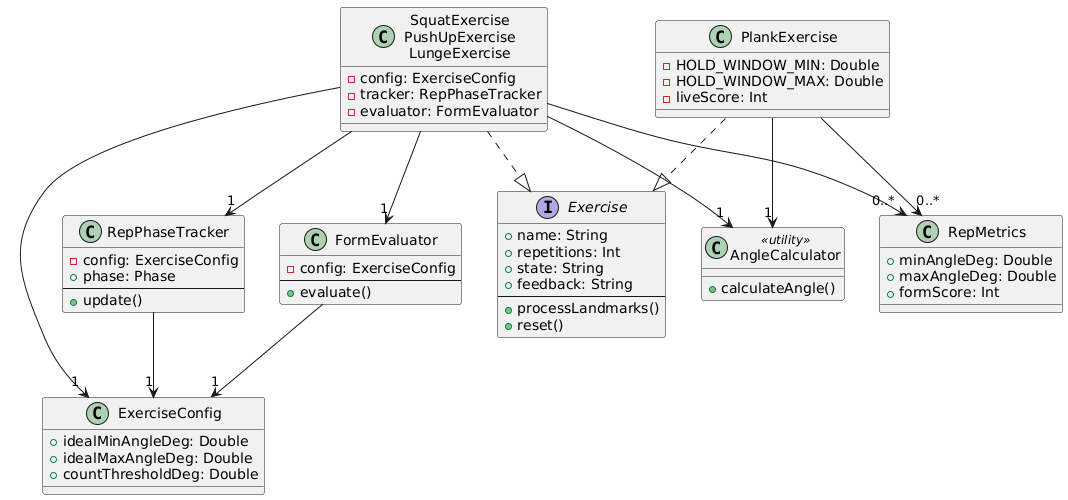
\includegraphics[width=\linewidth]{figuras/diagrama_avalição_forma.png}
   \caption{Diagrama de classes UML do motor de avaliação de exercícios}
   \label{fig:umlClasses}
\end{figure}

A orquestração do treino, por sua vez, é feita por duas \textit{Activities} distintas conforme o tipo de sessão: o \texttt{MainActivity} conduz planos multi-exercício definidos pelo utilizador através de um \texttt{WorkoutManager}, que percorre sequencialmente uma lista de \texttt{TrainingStep} (cada um associando um \texttt{Exercise} a uma meta de repetições ou de tempo, incluindo pausas via \texttt{RestExercise}); já o \texttt{ExerciseTestActivity} conduz uma sessão guiada de exercício único, com deteção de posição inicial (\texttt{StartPositionDetector}) e contagem decrescente antes de começar a contar repetições. Ambas partilham o \texttt{OverlayView} (esqueleto e HUD sobre a câmara) e o \texttt{TTSHelper} (indicações por voz). A Figura \ref{fig:umlOrquestracao} resume estas relações.

\pagebreak

\begin{figure}[h]
   \centering
   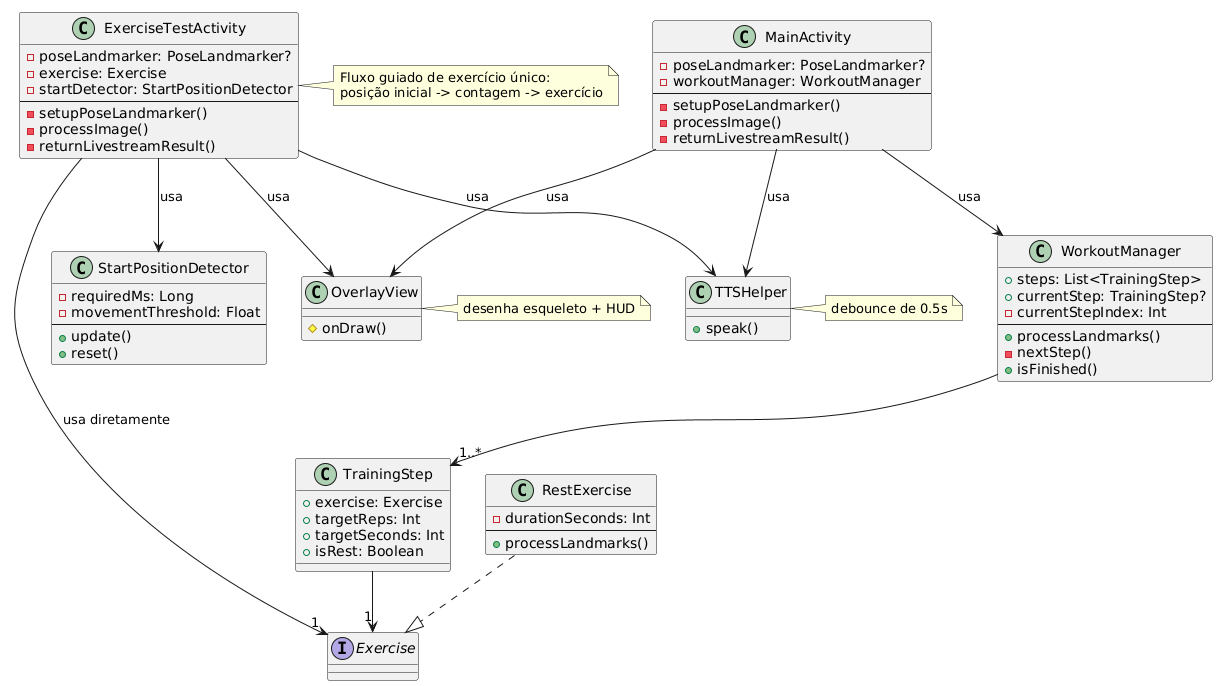
\includegraphics[width=\linewidth]{figuras/diagrama_treino.png}
   \caption{Diagrama de classes UML da orquestração do treino.}
   \label{fig:umlOrquestracao}
\end{figure}

O fluxo de navegação entre os ecrãs da aplicação (do \textit{login} ao resultado final de um treino) é apresentado no Apêndice \ref{ch:outroDetalheAdicional}, Figura \ref{fig:umlNavegacao}.

%%________________________________________________________________________
\section{Integração de Base de Dados e Gamificação}
\label{sec:integracaoDados}
%%________________________________________________________________________

Quando o utilizador conclui um treino, a aplicação calcula as calorias queimadas e executa uma escrita remota no Cloud Firestore:
\begin{itemize}
    \item Grava os dados do treino na coleção \texttt{/users/\{userId\}/workouts};
    \item Executa uma \textbf{Transação do Firestore} para atualizar de forma segura os campos \texttt{xpPoints} e \texttt{level} no perfil principal do utilizador. Desta forma, previne-se inconsistência de dados em escritas concorrentes.
\end{itemize}

A arquitetura NoSQL da aplicação distribui os dados numa hierarquia onde o documento do utilizador (\texttt{/users/\{userId\}}) guarda todos os agregados (Total de Calorias, Pontuação de Cadência Semanal, Pontos de Experiência), enquanto o registo intensivo e unitário de cada sessão repousa numa subcoleção aninhada (\texttt{/users/\{userId\}/workouts}). 

\begin{figure}[h]
   \centering
   \includegraphics[width=\linewidth]{figuras/datastrucutre.png}
   \caption{Diagrama da estrutura e esquema de dados.}
   \label{fig:umlClasses}
\end{figure}

\pagebreak

A decisão de executar a atualização dos campos agregados (\texttt{xpPoints}, \texttt{level}) em tempo de escrita, técnica conhecida como \textit{Write-Time Aggregation}, é uma boa prática em sistemas NoSQL escaláveis. Num protótipo com um reduzido número de utilizadores, a diferença de performance é impercetível; contudo, se a aplicação tiver de calcular a pontuação total do utilizador a partir de milhares de documentos iterados na coleção \texttt{workouts} a cada leitura, as \textit{queries} do Firebase tornar-se-ão progressivamente mais lentas e mais dispendiosas à medida que a coleção cresce (complexidade $O(N)$, linear no número de documentos lidos). Ao agregar os dados nativamente no momento em que a sessão é gravada, garantimos que qualquer funcionalidade concorrente (como as \textit{Leaderboards} globais do sistema de gamificação) acede a resultados definitivos numa leitura atómica $O(1)$.

% TODO : INSERIR AQUI A FIGURA 4.3 (PLACEHOLDER)
% \begin{figure}[H]
%     \centering
%     \includegraphics[width=0.8\textwidth]{figuras/FIGURA_LEADERBOARD_PLACEHOLDER.png}
%     \caption{Interface de Gamificação. ( ecrã das Leaderboards da app para demonstrar a eficácia da leitura em $O(1)$ de todos os utilizadores).}
%     \label{fig:gamificacao_leaderboard}
% \end{figure}


%%________________________________________________________________________
\chapter{Validação e Testes}
\label{ch:validacaoTestes}
%%________________________________________________________________________

A validação da aplicação foi realizada recorrendo a testes automatizados de compilação, simulações de base de dados e validações experimentais com utilizadores.

%%________________________________________________________________________
\section{Validação e Compilação Automatizada}
\label{sec:testesCompilacao}
%%________________________________________________________________________

A integridade do código fonte foi verificada através de \textit{builds} contínuos executados com a ferramenta Gradle:
\begin{itemize}
    \item \textbf{Compilação de Kotlin:} Executou-se a tarefa \texttt{compileDebugKotlin} para validar tipos estáticos e resolver dependências de bibliotecas de terceiros;
    \item \textbf{Geração de APK:} A tarefa \texttt{assembleDebug} empacotou com sucesso o ficheiro APK assinado para instalação e depuração física.
\end{itemize}


%%________________________________________________________________________
\section{Testes no Dispositivo e Limitações Físicas}
\label{sec:testesFisicos}
%%________________________________________________________________________

Uma limitação identificada nas ferramentas nativas do MediaPipe (PoseLandmarker) é o facto de compilarem binários nativos de partilha de código (\texttt{.so}) maioritariamente para a arquitetura ARM. 
Ao testar a aplicação em emuladores x86\_64 em sistemas Windows, a inicialização do pose landmarker falhava. O código foi robustecido com um bloco \texttt{try-catch} para desativar a câmara com segurança e mostrar um aviso ao programador/utilizador para correr a aplicação exclusivamente num dispositivo físico ARM. 

Em testes reais num smartphone físico moderno (Android 13, CPU Octa-core ARM), o processador local manteve uma taxa de frames de inferência estável próxima dos 25-30 FPS com tempo de computação de regras cinemáticas inferior a 1ms por frame, validando o modelo Edge Computing adotado.


%%________________________________________________________________________
\section{Validação de Analítica e Estado Social}
\label{sec:testesAnalitica}
%%________________________________________________________________________

Os testes de painel interativo e rede social cobriram:
\begin{itemize}
    \item \textbf{Seeding de Dados:} Testou-se a lógica de auto-seeding inserindo 5 treinos passados simulados. O painel estatístico em Jetpack Compose Canvas interpretou corretamente as datas e desenhou barras com altura proporcional às repetições completadas;
    \item \textbf{Limpeza de Histórico:} O botão "Clear History" eliminou de forma limpa todas as entradas na sub-coleção remota, atualizando instantaneamente os gráficos para o estado vazio;
    \item \textbf{Rede Social:} Validou-se a mecânica de aceitação de pedidos de amizade entre dois perfis distintos na consola Firebase, confirmando que a transação atómica adiciona os códigos correspondentes em simultâneo a ambos os utilizadores.
\end{itemize}


%%________________________________________________________________________
\section{Testes de Usabilidade e Validação Prática}
\label{sec:testesUsabilidade}
%%________________________________________________________________________

A validação da interface e da precisão do sistema em ambiente real foi conduzida através de testes de usabilidade estruturados. O protocolo envolveu 7 participantes, segmentados em três grupos com diferentes níveis de literacia tecnológica:
\begin{itemize}
    \item \textbf{Grupo A (Literacia Baixa - 2 participantes):} Foco na avaliação da autonomia inicial, compreensão do vocabulário da interface e dependência de apoio visual.
    \item \textbf{Grupo B (Literacia Média - 3 participantes):} Foco no teste de fluxos de treino padrão e calibração da câmara em ambientes domésticos restritos.
    \item \textbf{Grupo C (Literacia Avançada - 2 participantes):} Foco em testar os limites do algoritmo a ritmos elevados de execução e com utilizadores de estatura elevada (superiores a 1,90m).
\end{itemize}

A avaliação quantitativa recorreu à escala System Usability Scale (SUS), através de um questionário digital. Embora a amostra de utilizadores ($N=7$) seja estatisticamente reduzida, a intenção primordial desta avaliação não foi validar o sistema para lançamento em massa, mas sim obter um grupo de controlo preliminar que orientasse as decisões de desenvolvimento adotadas até à data. O \textit{score} global da aplicação obteve uma média de \textbf{66.42} pontos num máximo de 100 ($M = 66.42$, $SD = 19.62$), aproximando-se da média dita padrão da indústria (68 pontos), e expõe, em simultâneo, lacunas concretas no fluxo de utilização.

 \begin{figure}[H]
     \centering
     \includegraphics[width=0.55\textwidth]{figuras/SUS results.png}
     \caption{Distribuição dos resultados SUS por literacia tecnológica.}
     \label{fig:sus_results}
 \end{figure}

Contudo, a análise qualitativa transversal (observação direta das métricas de erro e entrevistas pós-treino) permitiu identificar pontos críticos que resultaram numa correção ágil da aplicação, concretizando as seguintes otimizações:
\begin{itemize}
    \item \textbf{Interface e Idioma:} A ausência de tradução (aplicação nativamente em inglês) gerou entropia e hesitação no ecrã de registo inicial, especialmente nos elementos mais envelhecidos do Grupo A. Em resposta direta, implementou-se um seletor de linguagem (\textit{Language Toggle}) suportado por \texttt{AppCompatDelegate}, localizando a interface em tempo real para \textit{pt-PT}.
    \item \textbf{Pacing do Feedback Sonoro (TTS):} Em ritmos elevados, o motor Text-to-Speech nativo do Android gerou sobreposição acústica (frases emitidas em simultâneo). Identificou-se a necessidade de um silêncio (debounce) forçado de 0.5 segundos entre instruções de voz, agora codificado na classe \texttt{TTSHelper}, para garantir a clareza do feedback sonoro.
    \item \textbf{Visibilidade Funcional à Distância:} À distância necessária para o enquadramento completo do esqueleto corporal do atleta (entre 2.5m a 4.1m), o texto do ecrã (HUD) tornou-se ilegível, induzindo quebras da postura lombar nos utilizadores que tentavam focar os olhos no visor. Por conseguinte, foi aplicada uma escala de redimensionamento às fontes de contexto e contagem (aumentadas até 150 pontos).
    \item \textbf{Fidelidade Cinemática por Oclusão (Lunges):} Enquanto os exercícios frontais de geometria aberta (Agachamentos e Flexões de Braços) demonstraram excelente robustez de leitura, os Afundos (\textit{Lunges}) apresentaram elevadas taxas de falha. Este falso negativo decorreu da oclusão visual da perna traseira face à perna da frente durante o plano lateral, o que corrompia os ângulos calculados a partir dessa perna. A correção não foi um algoritmo de deteção de oclusão, mas uma mudança mais direta: o sistema passou a identificar a cada frame qual a perna está à frente (pela posição horizontal dos pés) e a monitorizar o joelho dessa perna em vez do traseiro, eliminando o problema na origem em vez de o compensar. Esta mudança obrigou também a recalibrar os limiares de deteção (Secção \ref{sec:calibracaoLimiares}).
\end{itemize}

%%________________________________________________________________________
\section{Produto Final}
\label{sec:ProdutoFinal}
%%________________________________________________________________________

A consolidação da lógica de negócio cinemática com a camada de apresentação gráfica, aliada às correções iterativas impulsionadas pelo feedback dos testes SUS e observação direta, culminou numa \textit{final release} robusta e centrada no utilizador. Entre as otimizações implementadas nesta reta final, destaca-se a localização integral da interface para o idioma português, o que mitigou as entropias de navegação iniciais reportadas pelo grupo de teste.

Ao nível da usabilidade geral, a aplicação incorpora as diretrizes nativas de acessibilidade (incluindo navegação fluida em retrocesso e ações explícitas de \textit{Sign Off}), suportadas por um sistema de autenticação que exige confirmação por e-mail para a criação segura da conta. Na preparação da atividade (Figura \ref{fig:app_start}), o utilizador beneficia de um modelo flexível: é possível construir planos de treino inteiramente personalizados ou simplesmente iniciar planos pré-construídos, otimizando o tempo de preparação.

 \begin{figure}[H]
     \centering
     \includegraphics[width=0.4\textwidth]{figuras/StartingScreen.png}
     \caption{Ecrã de login e Menu inicial de seleção de treinos.}
     \label{fig:app_start}
 \end{figure}

A Figura \ref{fig:app_flow} ilustra o ciclo de vida completo de uma sessão de treino em ambiente real. Esta sequência demonstra a capacidade do sistema em guiar o utilizador de forma perfeitamente autónoma. Desde a calibração inicial até à transição automática entre exercícios e períodos de descanso, a interface providencia uma experiência contínua e imersiva.

 \begin{figure}[H]
     \centering
     \includegraphics[width=0.9\textwidth]{figuras/FinalProduct.jpeg}
     \caption{Ciclo de utilização da aplicação: Ecrã inicial, Execução do exercício (com HUD), Intervalo de descanso (Rest), Retoma do exercício e Painel de Resultados finais.}
     \label{fig:app_flow}
 \end{figure}

O último ecrã, detalhado na Figura \ref{fig:app_results}, materializa o sistema de gamificação, refletindo de imediato uma síntese dos resultados do plano. Este painel prova a viabilidade das decisões de arquitetura de dados (Secção 4.3): as transações de dados pré-computadas na escrita permitem uma leitura limpa e imediata dos dados em formato analítico. A métrica apresentada de Pontos de Experiência (XP) atua primariamente como um avaliador rigoroso da execução técnica do atleta, validando assim a eficácia do \textit{Edge Computing}. Adicionalmente, esta arquitetura deixa as portas abertas e alicerces escaláveis para uma rápida integração futura em lógicas competitivas de \textit{Leaderboard} e interação em rede social.

 \begin{figure}[H]
     \centering
     \includegraphics[width=0.4\textwidth]{figuras/Results Final.png}
     \caption{Ecrã de visualização de Resultados e Ranking de pontos.}
     \label{fig:app_results}
 \end{figure}


%%________________________________________________________________________
\chapter{Conclusões e Trabalho Futuro}
\label{ch:conclusoesTrabalhoFuturo}
%%________________________________________________________________________

Este trabalho demonstrou a viabilidade de desenvolver um assistente de fitness inteligente num smartphone convencional, sem hardware dedicado. A integração do MediaPipe para estimativa de pose local, aliada a uma máquina de estados em Kotlin e a feedback sonoro (Text-to-Speech), resultou num sistema autónomo capaz de avaliar a amplitude e cadência de exercícios físicos com base na literatura biomecânica.

A validação prática (Secção \ref{sec:testesUsabilidade}) alcançou um \textit{score} SUS de 66.42 e expôs limitações tratadas de forma iterativa, como a sobreposição áudio, as escalas de leitura do HUD e as falhas de deteção no Lunge por oclusão lateral.

Como perspetivas de evolução tecnológica, o trabalho futuro estrutura-se em duas grandes frentes: validação de usabilidade e expansão biomecânica. Numa ótica orientada ao mercado e à retenção de utilizadores, planeia-se conduzir testes A/B com novas amostras populacionais para otimizar a representação visual do esforço (HUD) e validar as novas mecânicas de gamificação. Adicionalmente, prevê-se a implementação de desafios competitivos em tempo real entre atletas na rede de amigos. Ao nível da fiabilidade algorítmica, será necessário submeter a nova heurística geométrica do Lunge a testes intensivos de oclusão e estudar soluções preditivas para enquadramentos de câmara não ortodoxos. Por fim, ambiciona-se suportar novos exercícios de membros superiores (como a flexão de bíceps) e expandir o motor de pose para a avaliação postural tridimensional completa (alinhamento ombros-anca-tornozelo), tirando partido da coordenada de profundidade $z$ já extraída nativamente pelo modelo MediaPipe.